
\begin{figure}
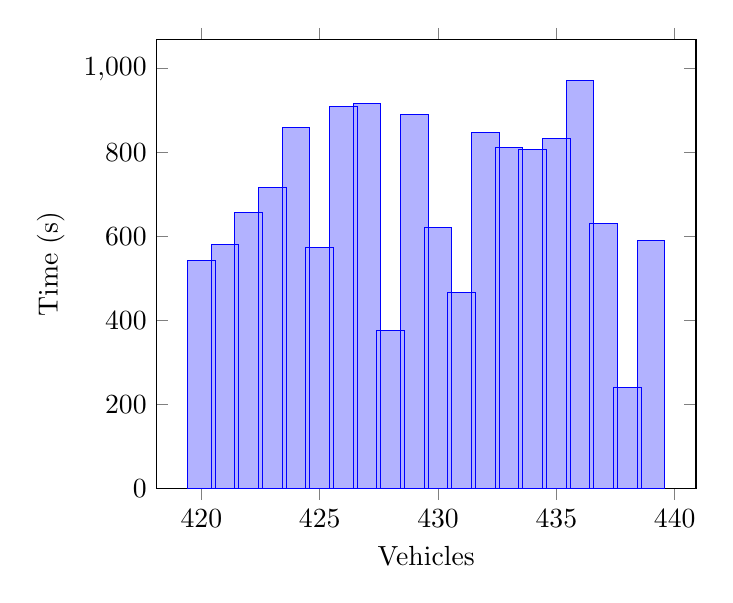
\begin{tikzpicture}
\begin{axis}[
legend style={anchor=west},
xlabel=Vehicles,
ylabel=Time (s),
ymin=0,
ybar,
]
\addplot coordinates {
(434, 807)
(424, 860)
(421, 581)
(435, 833)
(436, 972)
(420, 543)
(431, 466)
(423, 716)
(432, 848)
(426, 910)
(438, 240)
(422, 658)
(433, 813)
(439, 591)
(428, 375)
(430, 622)
(429, 892)
(427, 918)
(437, 630)
(425, 574)
};

\end{axis}
\end{tikzpicture}
\label{tik:time:100:65}
\caption{100 percent diving with GSC on route $65$}
\end{figure}
